\documentclass[border=4pt]{standalone}
\usepackage{amsmath}
\usepackage{tikz}
\usetikzlibrary{arrows.meta}

\begin{document}
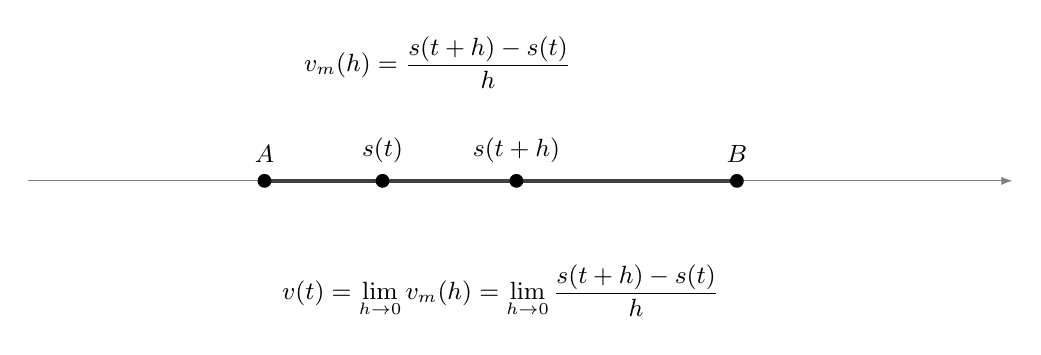
\begin{tikzpicture}[x=1cm, y=1cm, font=\small]
    \draw[-{Latex[length=4pt]}, gray] (0,0) -- (12.5,0);
    \draw[line width=1.6pt, black!75] (3,0) -- (9,0);
    \foreach \x/\l in {3/A, 4.5/s(t), 6.2/s(t+h), 9/B} {
        \fill (\x,0) circle (2.5pt);
        \node[above=3pt] at (\x,0) {$\l$};
    }
    \node at (5.2,1.5) {$v_{m}(h)=\dfrac{s(t+h)-s(t)}{h}$};
    \node at (6,-1.4) {$v(t)=\displaystyle\lim_{h\to 0}v_{m}(h)=\lim_{h\to 0}\dfrac{s(t+h)-s(t)}{h}$};
\end{tikzpicture}
\end{document}
